% ==========================================================================
% INFO 4617 Web Data Science -- Week 1: Introduction & Setup (Chapter 1)
% Build:  TEXINPUTS=../common: BIBINPUTS=../common: latexmk -pdf slides.tex
% (or run `make` from the slides/ directory)
%
% NOTE: The semester starts Thursday, Aug 20, so this week meets FRIDAY ONLY.
% This is a single-session intro deck, not the usual Mon/Wed/Fri shape.
% ==========================================================================
\documentclass[9pt,aspectratio=169]{beamer}
% ==========================================================================
% Shared preamble for INFO 4617 Web Data Science weekly lecture decks
% Based on the Gotham beamer theme (vendored in this directory).
% Each week's slides.tex does:  % ==========================================================================
% Shared preamble for INFO 4617 Web Data Science weekly lecture decks
% Based on the Gotham beamer theme (vendored in this directory).
% Each week's slides.tex does:  % ==========================================================================
% Shared preamble for INFO 4617 Web Data Science weekly lecture decks
% Based on the Gotham beamer theme (vendored in this directory).
% Each week's slides.tex does:  \input{preamble}  (with common/ on TEXINPUTS)
% then sets \title/\subtitle/\author/\date and \begin{document}.
% ==========================================================================

\usetheme{gotham}

\usepackage{fbb}
\usepackage{booktabs}
\usepackage{graphicx}
\usepackage{tikz}
\usepackage{xcolor}
\usepackage{multirow}
\usepackage{listings}
\usetikzlibrary{positioning, arrows.meta, shapes}

% Bibliography
\usepackage[style=authoryear,
            backend=biber,
            maxcitenames=1,
            uniquename=false,
            uniquelist=false]{biblatex}
\addbibresource{bibliography.bib}

\gothamset{sectiontocframe default=off}

% ------------------------------------------------------------------ colors
\definecolor{cugold}{HTML}{CFB87C}
\definecolor{tab-red}{HTML}{E15759}
\definecolor{tab-orange}{HTML}{F28E2B}
\definecolor{tab-blue}{HTML}{4E79A7}
\definecolor{tab-cyan}{HTML}{76B7B2}
\definecolor{tab-green}{HTML}{59A14F}
\definecolor{tab-yellow}{HTML}{EDC948}
\definecolor{tab-purple}{HTML}{B07AA1}
\definecolor{tab-pink}{HTML}{FF9DA7}
\definecolor{tab-brown}{HTML}{9C755F}
\definecolor{tab-gray}{HTML}{BAB0AC}

\setbeamercolor{frametitle}{fg=black, bg=cugold}
\setbeamercolor{progress bar}{fg=cugold, bg=cugold!20}

\setbeamercolor{block title alerted}{fg=black, bg=cugold}
\setbeamercolor{block body alerted}{fg=black, bg=cugold!10}

% ------------------------------------------------------------------ footline
\setbeamertemplate{footline}{
  \begin{beamercolorbox}[wd=\paperwidth,ht=2.5ex,dp=1ex,right]{footline}
    {\footnotesize \insertframenumber{} of \inserttotalframenumber}
    \hspace*{2ex}
  \end{beamercolorbox}
}

% ------------------------------------------------------------------ helpers
\newcommand{\bottomcite}[1]{
    \vspace*{\fill}
    \vspace{-\baselineskip}
    {\tiny
    \rule{\textwidth}{0.3pt}\\
    #1
    }
    \vspace{0.5ex}
}

% Consistent code styling for the Wednesday "applied notebook" frames.
\lstdefinestyle{wds}{
    basicstyle=\ttfamily\scriptsize,
    keywordstyle=\color{tab-blue}\bfseries,
    commentstyle=\color{tab-green},
    stringstyle=\color{tab-orange},
    showstringspaces=false,
    breaklines=true,
    columns=fullflexible,
    language=Python,
    aboveskip=0.4em,
    belowskip=0.4em,
}
\lstset{style=wds}

% \dayband{Day}{Topic} -- a lightweight section divider label used to mark
% Monday / Wednesday / Friday within a week's deck.
\newcommand{\dayband}[2]{{\large\textbf{#1}}\;\textcolor{tab-gray}{\textbar}\;#2}
  (with common/ on TEXINPUTS)
% then sets \title/\subtitle/\author/\date and \begin{document}.
% ==========================================================================

\usetheme{gotham}

\usepackage{fbb}
\usepackage{booktabs}
\usepackage{graphicx}
\usepackage{tikz}
\usepackage{xcolor}
\usepackage{multirow}
\usepackage{listings}
\usetikzlibrary{positioning, arrows.meta, shapes}

% Bibliography
\usepackage[style=authoryear,
            backend=biber,
            maxcitenames=1,
            uniquename=false,
            uniquelist=false]{biblatex}
\addbibresource{bibliography.bib}

\gothamset{sectiontocframe default=off}

% ------------------------------------------------------------------ colors
\definecolor{cugold}{HTML}{CFB87C}
\definecolor{tab-red}{HTML}{E15759}
\definecolor{tab-orange}{HTML}{F28E2B}
\definecolor{tab-blue}{HTML}{4E79A7}
\definecolor{tab-cyan}{HTML}{76B7B2}
\definecolor{tab-green}{HTML}{59A14F}
\definecolor{tab-yellow}{HTML}{EDC948}
\definecolor{tab-purple}{HTML}{B07AA1}
\definecolor{tab-pink}{HTML}{FF9DA7}
\definecolor{tab-brown}{HTML}{9C755F}
\definecolor{tab-gray}{HTML}{BAB0AC}

\setbeamercolor{frametitle}{fg=black, bg=cugold}
\setbeamercolor{progress bar}{fg=cugold, bg=cugold!20}

\setbeamercolor{block title alerted}{fg=black, bg=cugold}
\setbeamercolor{block body alerted}{fg=black, bg=cugold!10}

% ------------------------------------------------------------------ footline
\setbeamertemplate{footline}{
  \begin{beamercolorbox}[wd=\paperwidth,ht=2.5ex,dp=1ex,right]{footline}
    {\footnotesize \insertframenumber{} of \inserttotalframenumber}
    \hspace*{2ex}
  \end{beamercolorbox}
}

% ------------------------------------------------------------------ helpers
\newcommand{\bottomcite}[1]{
    \vspace*{\fill}
    \vspace{-\baselineskip}
    {\tiny
    \rule{\textwidth}{0.3pt}\\
    #1
    }
    \vspace{0.5ex}
}

% Consistent code styling for the Wednesday "applied notebook" frames.
\lstdefinestyle{wds}{
    basicstyle=\ttfamily\scriptsize,
    keywordstyle=\color{tab-blue}\bfseries,
    commentstyle=\color{tab-green},
    stringstyle=\color{tab-orange},
    showstringspaces=false,
    breaklines=true,
    columns=fullflexible,
    language=Python,
    aboveskip=0.4em,
    belowskip=0.4em,
}
\lstset{style=wds}

% \dayband{Day}{Topic} -- a lightweight section divider label used to mark
% Monday / Wednesday / Friday within a week's deck.
\newcommand{\dayband}[2]{{\large\textbf{#1}}\;\textcolor{tab-gray}{\textbar}\;#2}
  (with common/ on TEXINPUTS)
% then sets \title/\subtitle/\author/\date and \begin{document}.
% ==========================================================================

\usetheme{gotham}

\usepackage{fbb}
\usepackage{booktabs}
\usepackage{graphicx}
\usepackage{tikz}
\usepackage{xcolor}
\usepackage{multirow}
\usepackage{listings}
\usetikzlibrary{positioning, arrows.meta, shapes}

% Bibliography
\usepackage[style=authoryear,
            backend=biber,
            maxcitenames=1,
            uniquename=false,
            uniquelist=false]{biblatex}
\addbibresource{bibliography.bib}

\gothamset{sectiontocframe default=off}

% ------------------------------------------------------------------ colors
\definecolor{cugold}{HTML}{CFB87C}
\definecolor{tab-red}{HTML}{E15759}
\definecolor{tab-orange}{HTML}{F28E2B}
\definecolor{tab-blue}{HTML}{4E79A7}
\definecolor{tab-cyan}{HTML}{76B7B2}
\definecolor{tab-green}{HTML}{59A14F}
\definecolor{tab-yellow}{HTML}{EDC948}
\definecolor{tab-purple}{HTML}{B07AA1}
\definecolor{tab-pink}{HTML}{FF9DA7}
\definecolor{tab-brown}{HTML}{9C755F}
\definecolor{tab-gray}{HTML}{BAB0AC}

\setbeamercolor{frametitle}{fg=black, bg=cugold}
\setbeamercolor{progress bar}{fg=cugold, bg=cugold!20}

\setbeamercolor{block title alerted}{fg=black, bg=cugold}
\setbeamercolor{block body alerted}{fg=black, bg=cugold!10}

% ------------------------------------------------------------------ footline
\setbeamertemplate{footline}{
  \begin{beamercolorbox}[wd=\paperwidth,ht=2.5ex,dp=1ex,right]{footline}
    {\footnotesize \insertframenumber{} of \inserttotalframenumber}
    \hspace*{2ex}
  \end{beamercolorbox}
}

% ------------------------------------------------------------------ helpers
\newcommand{\bottomcite}[1]{
    \vspace*{\fill}
    \vspace{-\baselineskip}
    {\tiny
    \rule{\textwidth}{0.3pt}\\
    #1
    }
    \vspace{0.5ex}
}

% Consistent code styling for the Wednesday "applied notebook" frames.
\lstdefinestyle{wds}{
    basicstyle=\ttfamily\scriptsize,
    keywordstyle=\color{tab-blue}\bfseries,
    commentstyle=\color{tab-green},
    stringstyle=\color{tab-orange},
    showstringspaces=false,
    breaklines=true,
    columns=fullflexible,
    language=Python,
    aboveskip=0.4em,
    belowskip=0.4em,
}
\lstset{style=wds}

% \dayband{Day}{Topic} -- a lightweight section divider label used to mark
% Monday / Wednesday / Friday within a week's deck.
\newcommand{\dayband}[2]{{\large\textbf{#1}}\;\textcolor{tab-gray}{\textbar}\;#2}


\title[Week 1 · Introduction]{{\Huge Introduction \& Setup}}
\subtitle{Week 1 · Foundations module · Textbook Chapter 1}
\author[Keegan]{\textbf{Brian C. Keegan, Ph.D.} \\ Associate Professor, Department of Information Science \\ University of Colorado Boulder}
\date{Friday, August 21, 2026}

\begin{document}

\maketitle

% -------------------------------------------------------------------------
\begin{frame}{This week at a glance}
    \begin{columns}[T]
        \begin{column}{0.62\textwidth}
            Welcome to Web Data Science. The semester starts Thursday, so this week we meet \textbf{Friday only} --- today is orientation, setup, and the plan for the semester.

            \vspace{1em}

            \dayband{Friday}{Welcome, setup \& how the class works}
            \begin{itemize}\small
                \item What web data science is --- and why it matters
                \item Get Python, Git, and a GitHub account working
                \item How the weekly rhythm and grading work
            \end{itemize}

            \vspace{0.75em}

            The \textbf{Monday / Wednesday / Friday} rhythm begins next week --- see ``The weekly rhythm.''
        \end{column}
        \begin{column}{0.34\textwidth}
            \begin{block}{Companion notebook}
                \footnotesize \texttt{ch-01-introduction.ipynb}
            \end{block}
            \begin{alertblock}{Before Monday}
                \footnotesize Install Anaconda and create a \textbf{free} GitHub account. Bring a laptop --- we work hands-on.
            \end{alertblock}
        \end{column}
    \end{columns}
\end{frame}

% =========================================================================
\section{Welcome}
% =========================================================================

\begin{frame}{Meet your instructor}
    \begin{columns}[T]
        \begin{column}{0.6\textwidth}
            \textbf{Brian C. Keegan} --- Associate Professor of Information Science.
            \begin{itemize}\small
                \item Grew up outside Las Vegas, Nevada
                \item MIT: Mechanical Engineering and Science, Technology \& Society
                \item A year as a bartender and oral historian
                \item Ph.D.\ at Northwestern (Media, Technology \& Society); postdoc in computational social science at Northeastern
                \item Data scientist at Harvard Business School
                \item CU Boulder Information Science, 2016--present
            \end{itemize}
            \vspace{0.5em}
            {\footnotesize \texttt{brianckeegan.com}}
        \end{column}
        \begin{column}{0.36\textwidth}
            \begin{block}{What I study}
                \footnotesize
                \begin{itemize}\footnotesize
                    \item How Wikipedia covers breaking news
                    \item Public-interest data science
                    \item Migration across platforms (Threads, Mastodon, Bluesky)
                    \item Online extremism and moderation
                \end{itemize}
            \end{block}
            {\footnotesize My students and I rely on web data every day --- but researchers' access to it is rapidly disappearing.}
        \end{column}
    \end{columns}
\end{frame}

\begin{frame}{What is web data science?}
    \begin{columns}[T]
        \begin{column}{0.58\textwidth}
            \textbf{Web data science} is the practice of \textit{retrieving} data from the web, \textit{parsing} it into structured formats, and \textit{analyzing} it to produce knowledge.

            \vspace{1em}

            It differs from general data science in one crucial way: your first challenge is not modeling or visualization --- it is \textbf{getting the data in the first place}.

            \vspace{1em}

            The web is the largest, most dynamic, and most contested data source ever created. It can tell us how misinformation spreads, how housing costs shift, and how online communities govern themselves.
        \end{column}
        \begin{column}{0.38\textwidth}
            \begin{block}{Not your usual dataset}
                \footnotesize The web is \textbf{not a database}. Data arrives as:
                \begin{itemize}\footnotesize
                    \item HTML tables buried in tracking scripts
                    \item JSON from rate-limited APIs
                    \item scanned PDFs of council minutes
                    \item posts that might vanish tomorrow
                \end{itemize}
            \end{block}
        \end{column}
    \end{columns}
    \bottomcite{Textbook Ch.~1, ``Why Web Data Science?''}
\end{frame}

\begin{frame}{Data in the public interest}
    \begin{columns}[T]
        \begin{column}{0.58\textwidth}
            Web data science grew out of \textbf{computational social science}, \textbf{data journalism}, and \textbf{civic technology} --- traditions that share one idea: data fluency is a form of power that should serve the public.

            \vspace{0.75em}

            \begin{itemize}\small
                \item \textbf{ProPublica, ``Machine Bias'' (2016)} --- scraped court records exposed racial bias in criminal risk-assessment algorithms.
                \item \textbf{The Markup, ``Citizen Browser''} --- a recruited panel revealed how Facebook's feed distributed political content.
            \end{itemize}
        \end{column}
        \begin{column}{0.38\textwidth}
            \begin{alertblock}{The tools are not neutral}
                \footnotesize The same skills that make public information \textbf{accessible} can also enable surveillance. Who benefits? Who is harmed? These questions run through every chapter.
            \end{alertblock}
        \end{column}
    \end{columns}
    \bottomcite{Textbook Ch.~1, ``Social History \& Public Interest.'' The field's founding vision: \textcite{lazer2009computational}.}
\end{frame}

\begin{frame}{The loop that structures everything}
    \begin{columns}[T]
        \begin{column}{0.54\textwidth}
            Every chapter in this course follows the same arc:

            \vspace{0.75em}

            {\large \textbf{retrieve $\rightarrow$ parse $\rightarrow$ analyze}}

            \vspace{0.75em}

            \begin{itemize}\small
                \item \textbf{Retrieve} a page or API response with \texttt{requests}
                \item \textbf{Parse} it into records --- HTML, JSON, XML, or PDF
                \item Load into a \textbf{pandas} DataFrame
                \item \textbf{Analyze} or visualize the result
            \end{itemize}

            \vspace{0.75em}

            The specifics change; the arc does not. Recognizing it early gives you a mental model for every new chapter.
        \end{column}
        \begin{column}{0.42\textwidth}
            \centering
            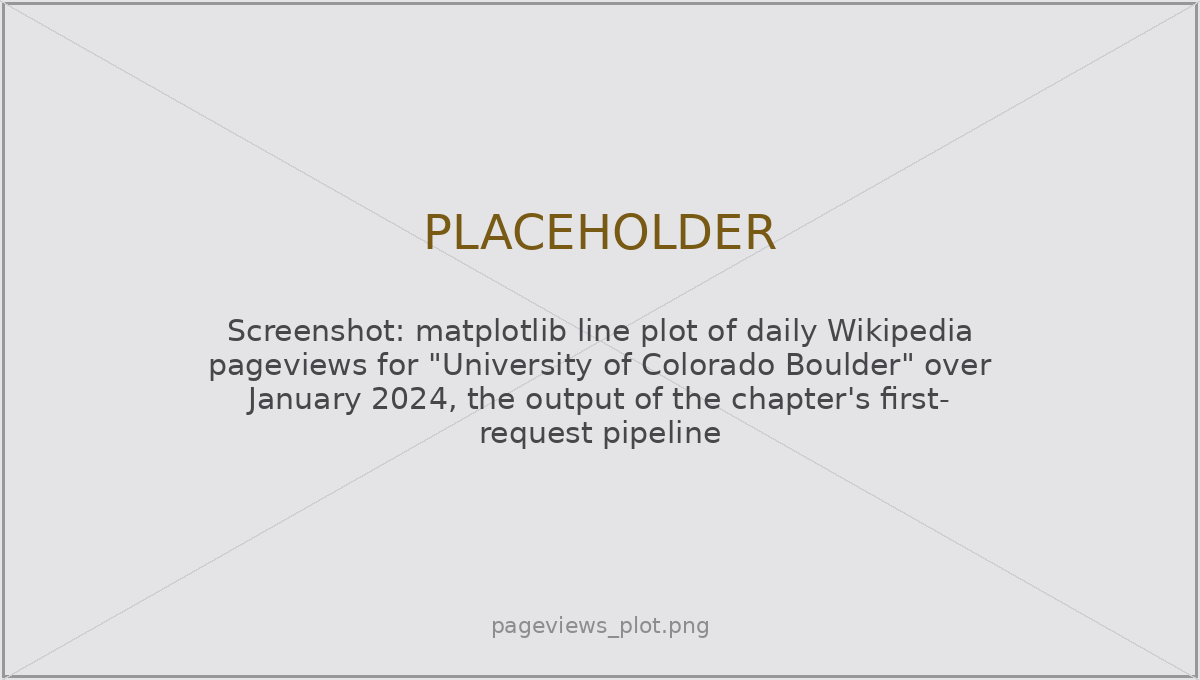
\includegraphics[width=\textwidth]{img/pageviews_plot.png}\\
            {\scriptsize A first pipeline: CU Boulder's daily Wikipedia pageviews.}
        \end{column}
    \end{columns}
    \bottomcite{Textbook Ch.~1, ``Your First Request.''}
\end{frame}

\begin{frame}{The data science mindset}
    Technical fluency is not enough. Four dispositions will serve you all semester:
    \begin{itemize}
        \item \textcolor{tab-green}{\textbf{Growth mindset}} --- ability develops through effort. Treat each error as a learning signal, not evidence of inadequacy.
        \item \textcolor{tab-blue}{\textbf{Computational thinking}} --- decompose, recognize patterns, abstract, and specify unambiguous steps \parencite{wing2006computational}.
        \item \textcolor{tab-orange}{\textbf{The hacker ethic}} --- sharing, openness, curiosity, and a bias toward action. The libraries you'll use exist because people shared their work.
        \item \textcolor{tab-purple}{\textbf{Scientific norms}} --- communalism, skepticism, and reproducibility. Document your methods; question your data; report limitations.
    \end{itemize}
    \vspace{0.5em}
    \begin{alertblock}{This is normal}
        \footnotesize You will meet libraries you've never used and pages that resist your parsing. Frustration is the job, not a detour from it.
    \end{alertblock}
    \bottomcite{Textbook Ch.~1, ``The Data Science Mindset.''}
\end{frame}

% =========================================================================
\section{How this class works}
% =========================================================================

\begin{frame}{The weekly rhythm}
    \begin{columns}[T]
        \begin{column}{0.56\textwidth}
            Starting next week, every week runs on the same three-beat rhythm:

            \vspace{0.75em}

            \dayband{Monday}{Concept + notebook intro}
            \begin{itemize}\small
                \item Read the chapter; I introduce the week's ideas and the companion notebook
            \end{itemize}
            \vspace{0.4em}
            \dayband{Wednesday}{Notebook lab}
            \begin{itemize}\small
                \item Hands-on --- we work and debug the chapter's code together, live
            \end{itemize}
            \vspace{0.4em}
            \dayband{Friday}{Textbook revisions}
            \begin{itemize}\small
                \item Propose and peer-review pull requests that improve the book
            \end{itemize}
        \end{column}
        \begin{column}{0.4\textwidth}
            \centering
            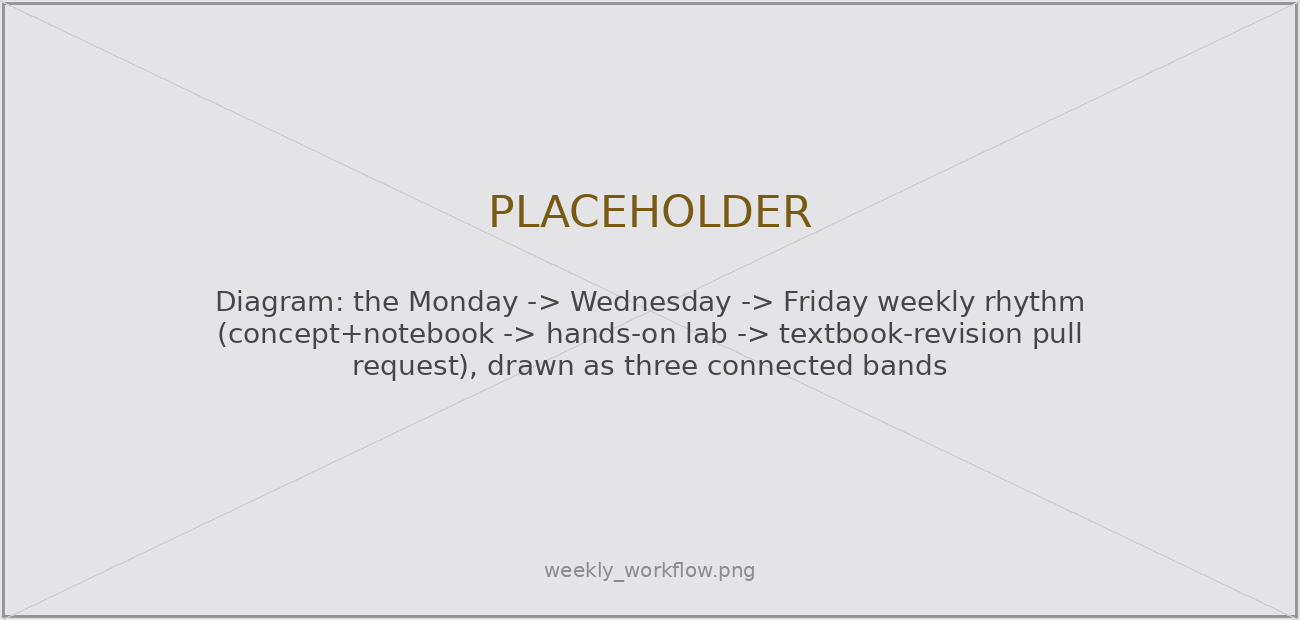
\includegraphics[width=\textwidth]{img/weekly_workflow.png}\\
            {\scriptsize Concept, then practice, then contribution.}
        \end{column}
    \end{columns}
    \bottomcite{This week is the exception --- Friday only. The full rhythm begins next week.}
\end{frame}

\begin{frame}{How you're evaluated}
    \begin{columns}[T]
        \begin{column}{0.54\textwidth}
            Your grade is \textbf{what you build}, not what you memorize:
            \vspace{0.5em}
            \begin{itemize}
                \item \textcolor{tab-blue}{\textbf{Notebook Labs --- 30\%}}\\ {\small weekly, hands-on data-collection work}
                \item \textcolor{tab-green}{\textbf{Textbook Revisions --- 30\%}}\\ {\small pull requests + peer reviews that improve the book}
                \item \textcolor{tab-orange}{\textbf{Final Project --- 40\%}}\\ {\small a research design + real data collection + analysis}
            \end{itemize}
        \end{column}
        \begin{column}{0.4\textwidth}
            \begin{block}{No exams}
                \footnotesize No midterm, no final. You demonstrate learning by \textbf{doing the work of a web data scientist} --- collecting data, contributing to a shared resource, and building a project.
            \end{block}
        \end{column}
    \end{columns}
    \bottomcite{Percentages are the course total; weekly labs are not individually high-stakes.}
\end{frame}

\begin{frame}{Documentation is the job}
    \begin{columns}[T]
        \begin{column}{0.58\textwidth}
            Your previous classes may have discouraged online resources. \textbf{The training wheels are off.} Finding, reading, and applying documentation is \textit{the} core professional skill --- not a shortcut, not cheating.

            \vspace{0.75em}

            Bookmark the docs you'll live in: \texttt{requests}, \texttt{BeautifulSoup}, \texttt{pandas}, \texttt{matplotlib}.

            \vspace{0.75em}

            ``It's not working'' is not a question. Say what you \textbf{tried}, what you \textbf{expected}, what \textbf{happened}, and what the \textbf{error message} says.
        \end{column}
        \begin{column}{0.38\textwidth}
            \begin{block}{Credit your sources}
                \footnotesize Used a blog post, a Q\&A answer, docs, or an AI tool to solve something beyond class?
                \vspace{0.3em}

                \textbf{Just include a link in your code.} Undocumented advanced tricks are a reliable signal of uncredited help.
            \end{block}
        \end{column}
    \end{columns}
    \bottomcite{Textbook Ch.~1, ``Documentation as Professional Practice.''}
\end{frame}

% =========================================================================
\section{Getting set up}
% =========================================================================

\begin{frame}{Three things you'll need}
    Before Monday, get all three working on your own laptop:
    \begin{enumerate}
        \item \textcolor{tab-blue}{\textbf{Python, via Anaconda}} --- the language plus a curated scientific stack and the \texttt{conda} package manager.
        \item \textcolor{tab-green}{\textbf{Git}} --- version control that tracks every change and lets many people edit the same project safely.
        \item \textcolor{tab-orange}{\textbf{A free GitHub account}} --- where our textbook lives and where you'll submit revisions as pull requests.
    \end{enumerate}
    \vspace{1em}
    \begin{alertblock}{Can't access a laptop or install software?}
        \footnotesize Contact me \textbf{immediately} so we can arrange an accommodation --- do not wait until an assignment is due.
    \end{alertblock}
\end{frame}

\begin{frame}[fragile]{Anaconda, environments \& core libraries}
    \begin{columns}[T]
        \begin{column}{0.56\textwidth}
            Install Anaconda from \texttt{anaconda.com}, then give this course its own isolated environment:
\begin{lstlisting}
conda create -n webdata python=3.11
conda activate webdata
pip install requests beautifulsoup4 \
    pandas matplotlib seaborn
\end{lstlisting}
            One environment per project records \textbf{exactly} which versions your analysis ran against --- reproducibility, not just tidiness.

            \vspace{0.5em}

            Launch your workspace with \texttt{jupyter notebook}: code, notes, and results in one file.
        \end{column}
        \begin{column}{0.4\textwidth}
            \centering
            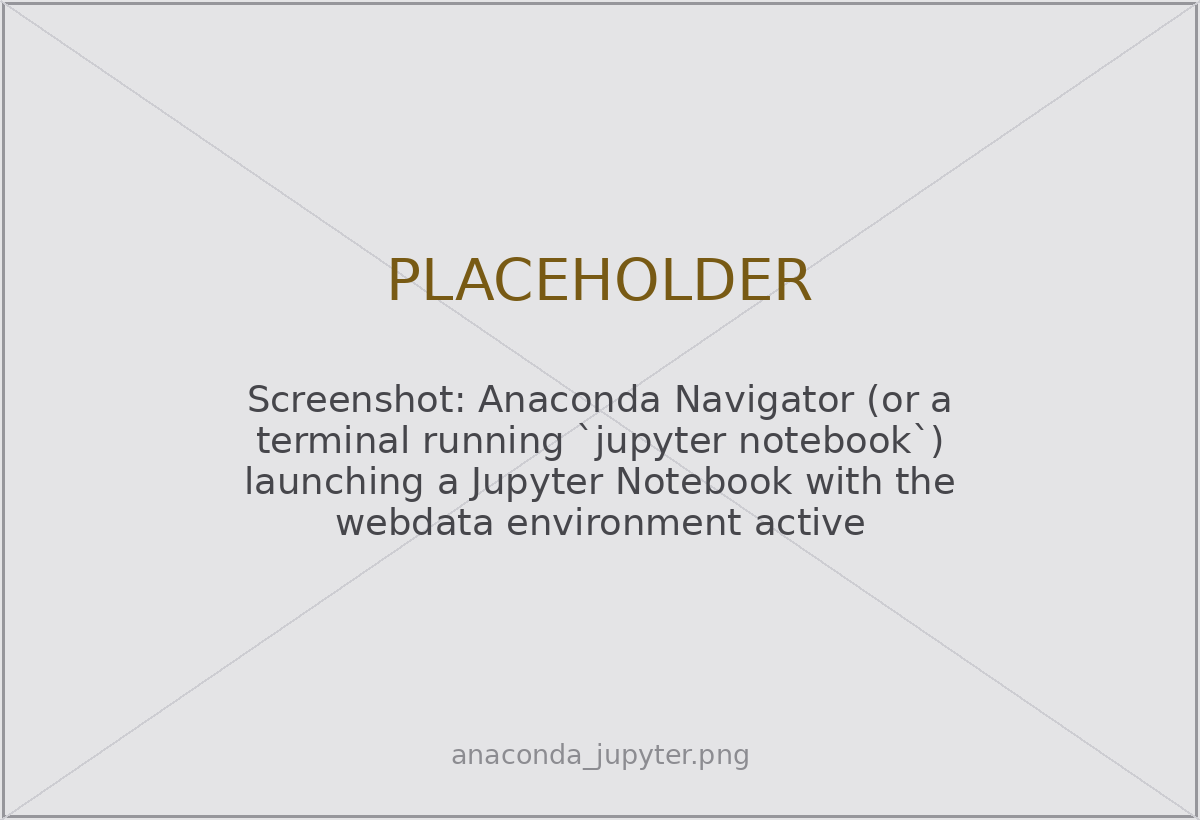
\includegraphics[width=\textwidth]{img/anaconda_jupyter.png}\\
            {\scriptsize Anaconda launches Jupyter in your browser.}
        \end{column}
    \end{columns}
    \bottomcite{Textbook Ch.~1, ``Setting Up Your Environment.'' No spreadsheets or BI tools (Excel, Tableau) for coursework.}
\end{frame}

\begin{frame}[fragile]{Your first request}
    Retrieving a web page programmatically is as simple as one call. Confirm your setup works:
\begin{lstlisting}
import requests

url = "https://en.wikipedia.org/wiki/University_of_Colorado_Boulder"
response = requests.get(url)

print(response.status_code)   # 200 means success
print(len(response.text))     # characters of raw HTML
\end{lstlisting}
    Raw HTML isn't data yet. An API hands back JSON that drops straight into a DataFrame:
\begin{lstlisting}
import pandas as pd
api = "https://wikimedia.org/api/rest_v1/metrics/pageviews/per-article"
url = f"{api}/en.wikipedia/all-access/all-agents/{article}/daily/20240101/20240131"
headers = {"User-Agent": "WebDataScience/1.0 (you@colorado.edu)"}

data = requests.get(url, headers=headers).json()  # JSON -> dict
df = pd.DataFrame(data["items"])                   # list of dicts -> DataFrame
\end{lstlisting}
    \bottomcite{Textbook Ch.~1, ``Your First Request.'' The \texttt{User-Agent} header identifies you --- a politeness norm we revisit next week.}
\end{frame}

\begin{frame}{Git \& a free GitHub account}
    \begin{columns}[T]
        \begin{column}{0.56\textwidth}
            \textbf{Git} records the history of a project --- who changed what, when, and why --- and lets many people work on it without overwriting each other.

            \vspace{0.75em}

            \textbf{GitHub} hosts Git projects online. Create a free account at \texttt{github.com}. Our textbook lives there as an open repository:

            \vspace{0.4em}
            {\footnotesize \texttt{github.com/cuinfoscience/Web-Data-Science-Book}}
            \vspace{0.4em}

            You'll \textbf{fork} it (make your own copy), edit a chapter, and propose your change back --- exactly how open-source software is built.
        \end{column}
        \begin{column}{0.4\textwidth}
            \centering
            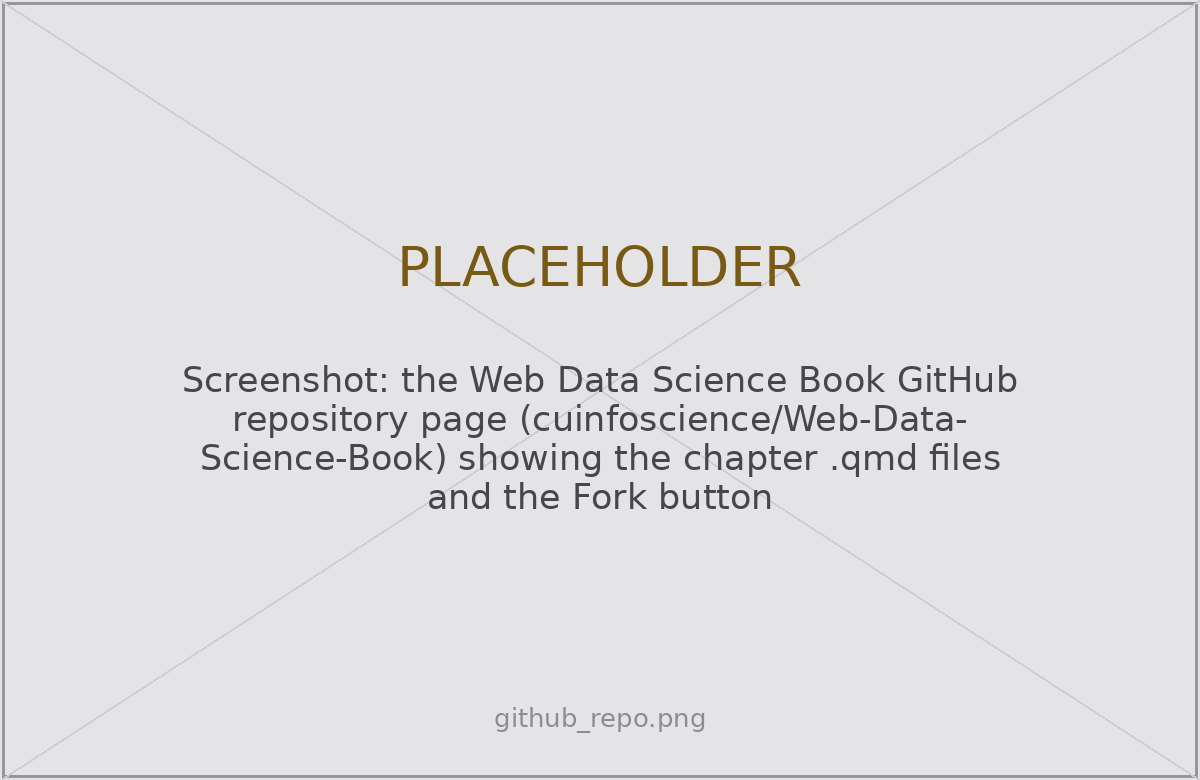
\includegraphics[width=\textwidth]{img/github_repo.png}\\
            {\scriptsize The book is a living, open repository.}
        \end{column}
    \end{columns}
    \bottomcite{Sign up with your \texttt{colorado.edu} email to unlock free student features.}
\end{frame}

\begin{frame}{Textbook revisions as pull requests}
    \begin{columns}[T]
        \begin{column}{0.58\textwidth}
            Every Friday you improve the book itself. The workflow you'll repeat all semester:
            \begin{enumerate}\small
                \item \textbf{Fork / branch} the book repository
                \item \textbf{Edit} a chapter's \texttt{.qmd} source; commit with a clear message
                \item \textbf{Open a pull request} describing \textit{what} you changed and \textit{why}
                \item \textbf{Review} two classmates' PRs --- kind, specific, and actionable
            \end{enumerate}

            \vspace{0.5em}

            A pull request is a proposal: your change sits side-by-side with the original so peers and I can comment line-by-line before it merges.
        \end{column}
        \begin{column}{0.38\textwidth}
            \centering
            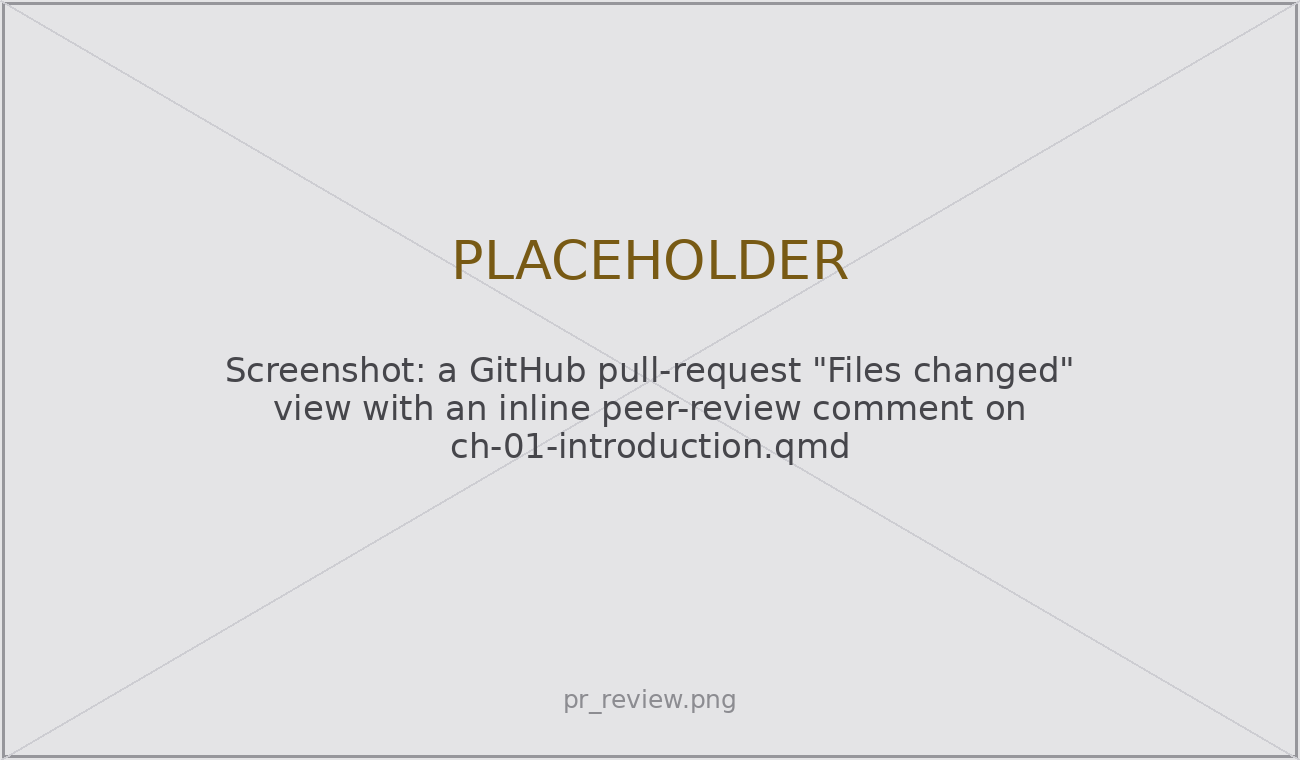
\includegraphics[width=\textwidth]{img/pr_review.png}
        \end{column}
    \end{columns}
    \bottomcite{Contributions \& reviews count toward the Textbook Revisions grade (30\%). We walk through a real PR in Week~2.}
\end{frame}

\begin{frame}[standout]
    The web is not a database.\\
    It's a chaotic, evolving ecosystem of documents, APIs, and norms.\\[1em]
    {\large Your first challenge isn't modeling ---\\ it's getting the data at all.}
\end{frame}

% =========================================================================
\begin{frame}{Key takeaways}
    \begin{enumerate}
        \item Web data science is \textbf{retrieve $\rightarrow$ parse $\rightarrow$ analyze} --- and the hard part is getting the data at all.
        \item Every week has a rhythm: \textbf{Monday} concept, \textbf{Wednesday} notebook lab, \textbf{Friday} textbook-revision pull requests.
        \item Your grade is what you build: Labs 30\%, Revisions 30\%, Final Project 40\% --- \textbf{no exams}.
        \item Before Monday: install \textbf{Anaconda}, set up \textbf{Git}, and create a free \textbf{GitHub} account.
        \item Documentation is a professional skill, not a shortcut --- it's how you'll learn every new library.
    \end{enumerate}
    \vspace{0.75em}
    \centering\small Next week: \textbf{Ethics, law \& responsible collection} --- \texttt{robots.txt}, Terms of Service, and how to collect data without doing harm.
    \bottomcite{Reading: Textbook Ch.~1. Related: \textcite{salganik2018bit}; \textcite{wilson2017good}.}
\end{frame}

\end{document}
